\begin{enumerate}[label=\thesection.\arabic*.,ref=\thesection.\theenumi]
\numberwithin{equation}{enumi}

\item A second-order real system has the following properties:

a) the damping ratio $\zeta=0.5$ and undamped natural frequency $\omega_n=10rad/s$ 

b) the steady state value of the output, to a unit step input, is 1.02.

The transfer function of the system is\newline
(A) $\frac{1.02}{s^2+5s+100}$    (B) $\frac{102}{s^2+10s+100}$\newline
(C) $\frac{100}{s^2+10s+100}$  (D) $\frac{102}{s^2+5s+100}$ \newline
\solution Characteristic equation of second order system is as follows
\newline
\begin{align}
s^2+2\zeta\omega_ns+\omega_n^2=0
\end{align}
Given
\begin{align}
\zeta=0.5
\\
\omega_n=10rad/s
\end{align}
The damping coefficient is between 0 and 1. Thus, the system is Underdamped.

and the Characteristic equation becomes 
\begin{align}
 s^2+10s+100=0   
\end{align}
Denominator of the Transfer Function is characteristic equation. Considering this, we can eliminate A and D options.\newline

We know that output of the system in s domain is
\begin{align}\\
C(s)=T(s)R(s)
\\
R(s)=\frac{1}{s}
\end{align}
as it is unit step input.\newline

Steady state output is given by
\begin{align}
    C(\infty)=\lim_{s \to 0}sC(s)
\end{align}
Given, steady state output is 1.02 and is the same for only option B\newline

Therefore, transfer function of the system is
\begin{align}
    \frac{102}{s^2+10s+100}
\end{align}
The step response of the transfer function 
\begin{align}
    C(t)=\mathscr{L}^{-1}\cbrak{\frac{102}{s(s^2+10s+100)}}
\end{align}
Dividing into partial fractions
\begin{align}
C(t)=\mathscr{L}^{-1}\cbrak{\frac{51}{50s}}-\mathscr{L}^{-1}\cbrak{\frac{-51s-510}{50(s^2+10s+100)}}
\end{align}
\begin{align}
&C(t)=\brak{\frac{-51}{50}}\mathscr{L}^{-1}\cbrak{\frac{s+5}{(s+5)^2+75}}\nonumber\\
&+\brak{\frac{-51}{10}}\mathscr{L}^{-1}\cbrak{\frac{1}{(s+5)^2+75}}+\mathscr{L}^{-1}\cbrak{\frac{51}{50s}}
\end{align}
\newline

Applying Inverse Laplace Transform, we get
\begin{align}
\mathscr{L}^{-1}\cbrak{\frac{s+5}{(s+5)^2+75}}\nonumber\\
&=\exp^{-5t}cos(5\sqrt{3}t)
    \\
\mathscr{L}^{-1}\cbrak{\frac{1}{(s+5)^2+75}}=\nonumber\\&\frac{1}{5\sqrt{3}}\exp^{-5t}cos(5\sqrt{3}t)
\end{align}
\newline

Therefore,
\begin{align}
C(t)=&\brak{\frac{-51}{50}}\exp^{-5t}cos(5\sqrt{3}t)\nonumber\\
&-\brak{\frac{17\sqrt{3}}{50}}\exp^{-5t}sin(5\sqrt{3}t)+\frac{51}{50}u(t)
\end{align}
The following code is used to get the step response plot
\begin{lstlisting}
stepresponseplot.py
\end{lstlisting}
\begin{figure}
\centering
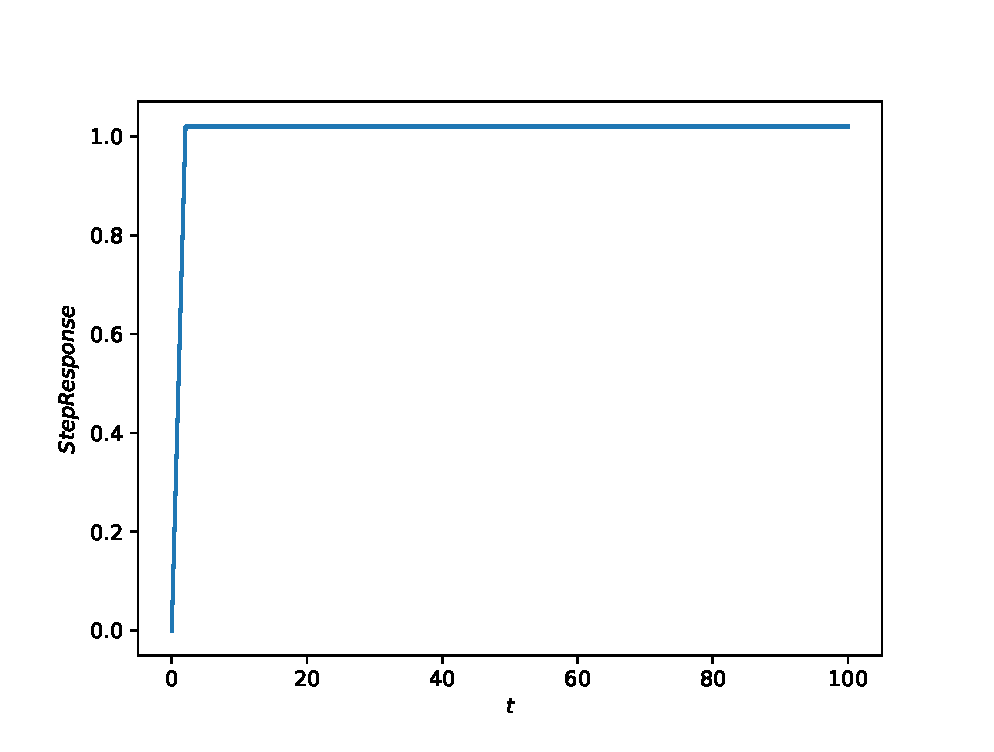
\includegraphics[width=\columnwidth]{./plot.eps}
\caption{}
\label{fig:sec_order}
\end{figure}
\end{enumerate}
